\section{Tombstone Diagram}
When crafting a compiler tombstone diagrams can be used to define the programming languages needed to compile the source code of a program. The tombstone diagram shows a program written in some programming language, which programming language the compiler is written in, and what the target language is.

\begin{figure}[H]
	\centering
		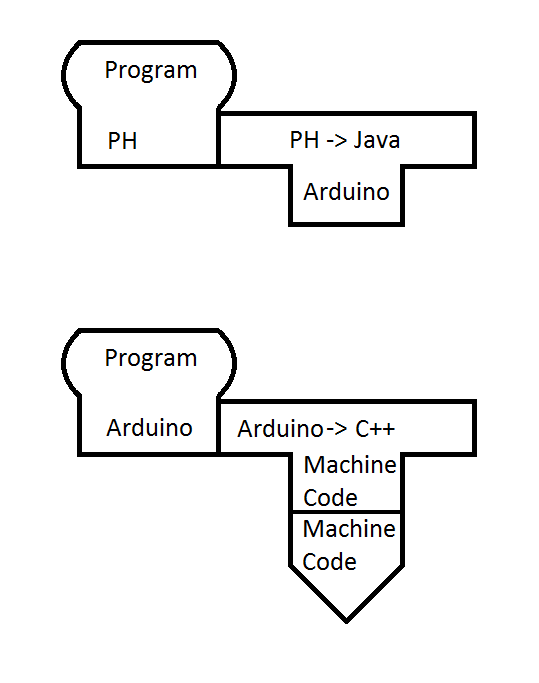
\includegraphics{billeder/tombstone_diagram.png}
		\caption{Tombstone diagram for the source language to machine code}
		\label{fig:tombstone}
\end{figure}

As seen in figure \ref{fig:tombstone} the tombstone diagram for this project is as follows: The program is written in PH \todo{Name for source language placeholder}, which is with the use of a compiler written in java translated to Arduino language. Arduino only understands machine code, so another compiler is needed to translate from Arduino language into machine code using a compiler written in java. (This compiler is the software Arduino has available through their website)
Since this project focuses on compiling from PH to Arduino language the first tombstone diagram in figure \ref{fig:tombstone} is the important one to notice.